% RESETEAR LOS CONTADORES PARA LOS ANEXOS
\setcounter{chapter}{1}
\setcounter{section}{0}
%%%%%%%%

\anx{I}{Guía de instalación}
\noindent
La aplicación en su conjunto, como se ha mencionado en anteriores puntos de esta memoria, consta de varios sistemas, desde la lógica de la aplicación hasta las llamadas a las diferentes APIs que ésta usa.

Para cada uno de estos sistemas, es necesario una configuración y despliegue específicos, es por ello que en este anexo se muestra cómo proceder a desplegar todos los entornos necesarios para el correcto funcionamiento de la aplicación.

\section{Instalación y despliegue del servidor Spring Boot}
Como ya se mencionó en el capítulo \ref{spring_boot_tool}, las peticiones que los administradores mandan a los endpoints de la API en Spring se utilizan tanto para la creación de nuevos usuarios como para realizar cambios en el correo electrónico y/o contraseña de éstos.

% AÑADIR AQUI REFERENCIAS A LA BIBLIOGRAFIA DE MAVEN Y GRADLE
En primer lugar cabe destacar que para desplegar el servidor de Spring se puede utilizar Maven o Gradle.\\
\textbf{\textit{Maven}} \cite{maven} ha sido y es una de las herramientas más populares para la gestión y construcción de proyectos en Java, utilizando conceptos provenientes de Apache Ant. La configuración de un proyecto utilizando Maven se basa en un fichero \texttt{.xml} en el cual se declaran los diferentes requerimientos (como las dependencias) para la construcción.\\
Por otro lado, \textbf{\textit{Gradle}} \cite{gradle} es una herramienta de automatización de compilación de código abierto que no emplea lenguaje XML como Maven, sino que se basa en un lenguaje específico del dominio (DSL) basado en Groovy \cite{groovy}.\\
Existen algunas diferencias entre Maven y Gradle, como el tiempo de construcción que en Gradle es más corto y rápido que en Maven; o los scripts, Maven utiliza XML lo que hace que los scripts sean más largos en comparación con los de Gradle, que son más cortos y limpios. Son estas las razones principales por las que se ha decidido emplear Gradle para la compilación, por lo que las instrucciones se realizarán basándose en la utilización de Gradle.

Para proceder al despliegue de este servidor es necesario tener localmente el proyecto de Spring, que se puede conseguir clonando el repositorio de este proyecto. Posteriormente, es necesario tener instalada la versión más reciente de Gradle y se deberá de añadir a las variables de entorno.\\
Luego se deben de añadir las dependencias necesarias de Google Firebase para el correcto funcionamiento, quedando un script similar al mostrado en la Figura \ref{fig:gradle_script}.

\begin{figure}[H]
    \centering
    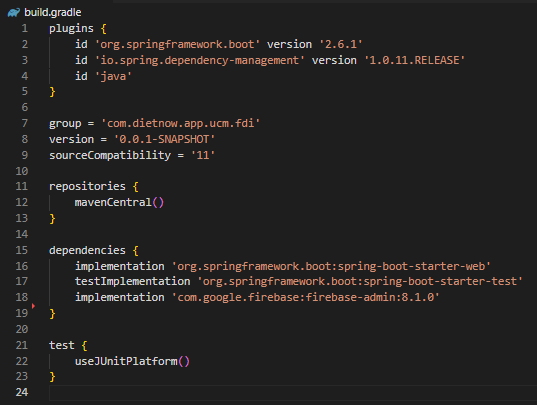
\includegraphics[width=0.8\textwidth]{Images/Annexes/gradle.png}
    \caption{Script de Gradle}
    \label{fig:gradle_script}
\end{figure}

Para compilar y ejecutar el servidor de Spring se deberá ejecutar el comando ``\texttt{gradlew bootRun}``, el cuál mostrará una salida como la de la Figura \ref{fig:gradle}:
\begin{figure}[H]
    \centering
    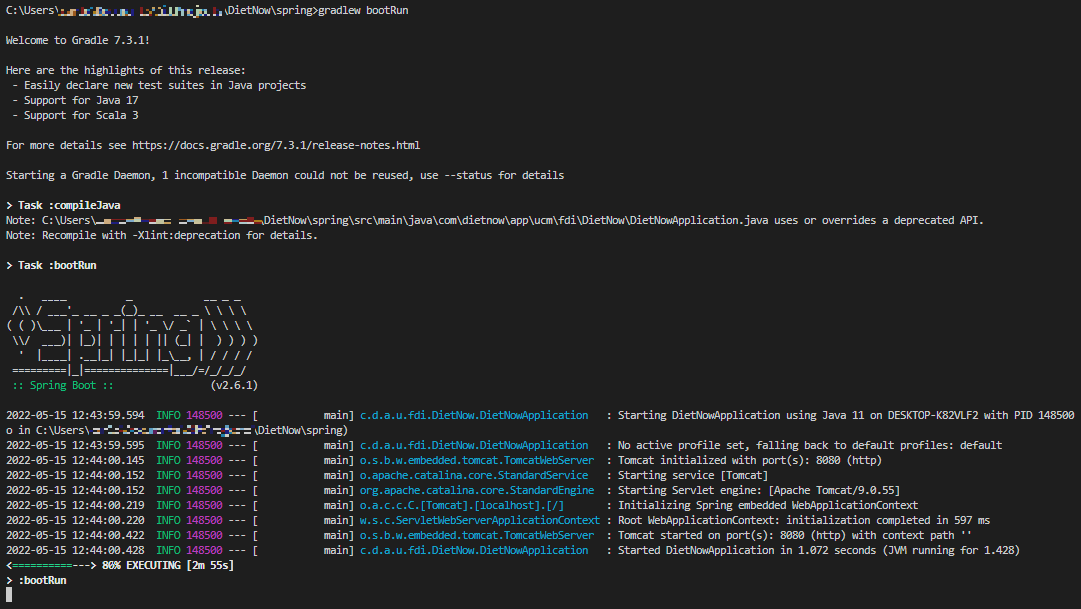
\includegraphics[width=\textwidth]{Images/Annexes/gradle_commandline.png}
    \caption{Ejecución de Gradle}
    \label{fig:gradle}
\end{figure}



\section{Instalación y despliegue del servidor Node.js}
El despliegue de este servidor es necesario para poder obtener la información nutricional de los diferentes alimentos dado el código de barras del mismo.

% AÑADIR AQUI REFERENCIAS A LA BIBLIOGRAFIA DE NODE
Para poder ejecutar y desplegar este servidor, es necesario tener instalada una versión actualizada de Node.js. En este caso no es necesaria ninguna dependencia externa adicional ya que las peticiones que se solicitan a la API de Open Food Facts se realizan mediante el módulo \texttt{https} ya implementado en Node.js por defecto. Para tener de forma local este proyecto de Node.js, se puede conseguir clonando el repositorio de este proyecto.

Posteriormente y, en la raíz del proyecto de Node.js, se deberá de ejecutar por línea de comandos en la terminar el comando ``\texttt{node index.js}``.\\
Para comprobar el correcto despliegue, se puede realizar una petición a esta API accediendo a la url ``\texttt{http://localhost:3000/dietnow/api/product/?barcode=XXXXXXXX}`` en el navegador para obtener la información nutricional del producto solicitado mediante el código de barras especificado, produciendo una salida similar a la mostrada en la Figura \ref{fig:node}.

\begin{figure}[H]
    \centering
    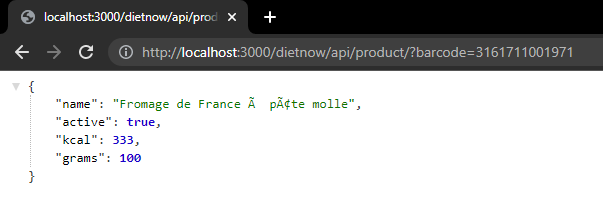
\includegraphics[width=\textwidth]{Images/Annexes/node.png}
    \caption{Producto solicitado a la API de Node.js}
    \label{fig:node}
\end{figure}